% chktex-file 1
% chktex-file 13
% chktex-file 24
% chktex-file 36
\section{Mục tiêu thực nghiệm}

Mục tiêu của quá trình thực nghiệm là đánh giá tính đúng đắn và hiệu quả của cơ chế hỗ trợ đối tượng \texttt{std::atomic} được bổ sung vào công cụ AKAUTAUTO. Thực nghiệm tập trung kiểm chứng khả năng của hệ thống trong việc nhận diện chính xác các biến có kiểu \texttt{std::atomic}, xây dựng cây dữ liệu kiểm thử tương ứng và sinh mã kiểm thử có thể biên dịch, thực thi thành công.

Bên cạnh đó, thực nghiệm đánh giá tính chính xác của lớp \texttt{AtomicDataNode} trong việc biểu diễn dữ liệu nguyên tử, cho phép người dùng cấu hình giá trị kiểm thử và sinh mã khởi tạo phù hợp trong test driver. Một mục tiêu quan trọng khác là kiểm chứng cơ chế xử lý các thao tác \texttt{load()} và \texttt{store()} trong quá trình sinh mã kiểm thử, bảo đảm các đoạn mã được sinh ra tuân thủ ngữ nghĩa của \texttt{std::atomic}.

Cuối cùng, thực nghiệm đánh giá mức độ cải thiện về khả năng kiểm thử thông qua các chỉ số độ phủ mã nguồn. Kết quả thu được được sử dụng để xác nhận rằng giải pháp đề xuất giúp mở rộng phạm vi hỗ trợ của AKAUTAUTO đối với các chương trình C/C++ sử dụng đối tượng nguyên tử.

\section{Cài đặt công cụ}

Công cụ được cài đặt và tích hợp dựa trên kiến trúc hiện có của AKAUTAUTO. Kiến trúc tổng quan của hệ thống bao gồm năm mô-đun chính: mô-đun xây dựng môi trường kiểm thử, mô-đun phân tích mã nguồn, mô-đun sinh dữ liệu kiểm thử, mô-đun thực thi và phân tích ca kiểm thử, và mô-đun sinh báo cáo kết quả. Trong phạm vi đề tài này, các cải tiến tập trung vào mô-đun phân tích mã nguồn, cây dữ liệu kiểm thử và cơ chế sinh test driver cho đối tượng \texttt{std::atomic}.

\begin{figure}[H]
    \centering
    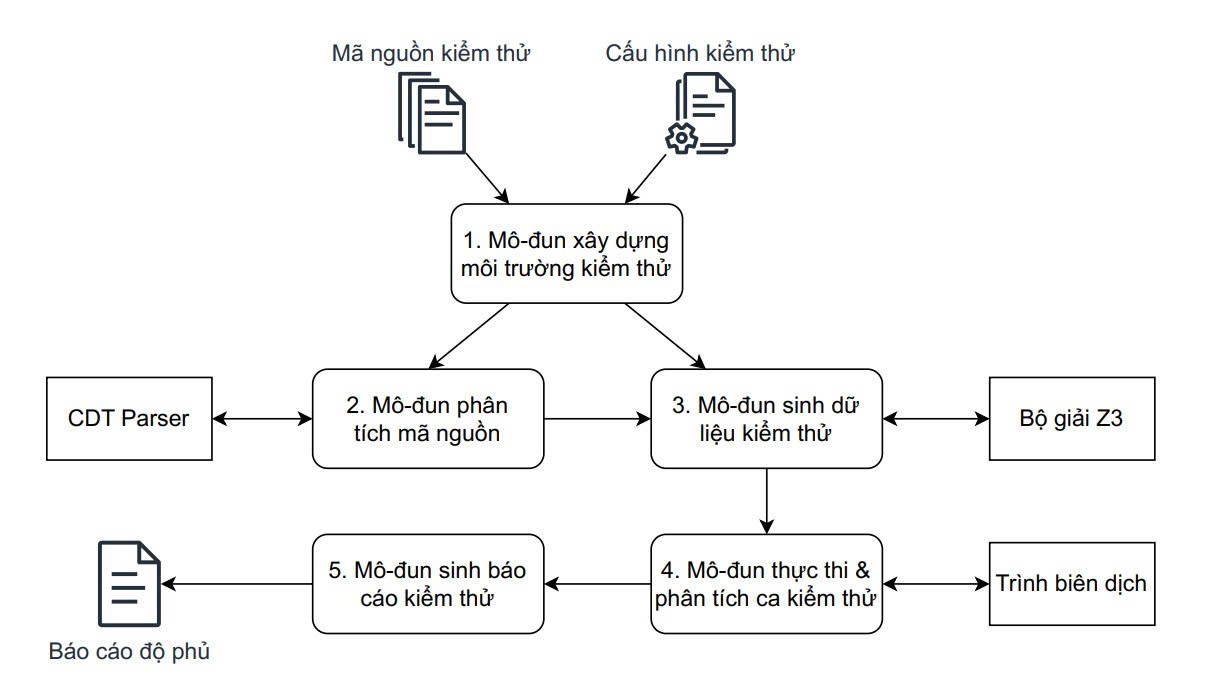
\includegraphics[width=0.95\linewidth]{images/image.png}
    \caption{Kiến trúc công cụ AKAUTAUTO}
    \label{fig:akautauto_architecture}
\end{figure}

\section[Công cụ AKAUTAUTO sau khi hỗ trợ \texttt{std::atomic}]{Công cụ AKAUTAUTO sau khi hỗ trợ\\\texttt{std::atomic}}

Sau khi bổ sung cơ chế hỗ trợ đối tượng \texttt{std::atomic}, kiến trúc tổng thể của công cụ AKAUTAUTO vẫn được giữ nguyên, tuy nhiên khả năng xử lý các chương trình C++ sử dụng kiểu dữ liệu nguyên tử đã được mở rộng. Các thành phần cốt lõi như bộ phân tích mã nguồn, cây dữ liệu kiểm thử (Data Tree), bộ sinh test driver và mô-đun đánh giá độ phủ vẫn được kế thừa từ phiên bản trước. Những thay đổi chủ yếu tập trung vào quá trình nhận diện kiểu dữ liệu và sinh mã kiểm thử cho các đối tượng \texttt{atomic}.

Cụ thể, mô-đun phân tích mã nguồn đã được mở rộng để nhận diện các biến có kiểu \texttt{std::atomic} với kiểu dữ liệu cơ sở tương ứng trong quá trình duyệt cây cú pháp trừu tượng (AST). Sau khi phát hiện kiểu dữ liệu nguyên tử, hệ thống tự động ánh xạ đối tượng sang lớp \texttt{AtomicDataNode} trong cây dữ liệu kiểm thử. Điều này cho phép các đối tượng \texttt{atomic} được quản lý và cấu hình dữ liệu đầu vào tương tự các kiểu dữ liệu đã được hỗ trợ trong hệ thống.

\begin{figure}[htbp]
    \centering
    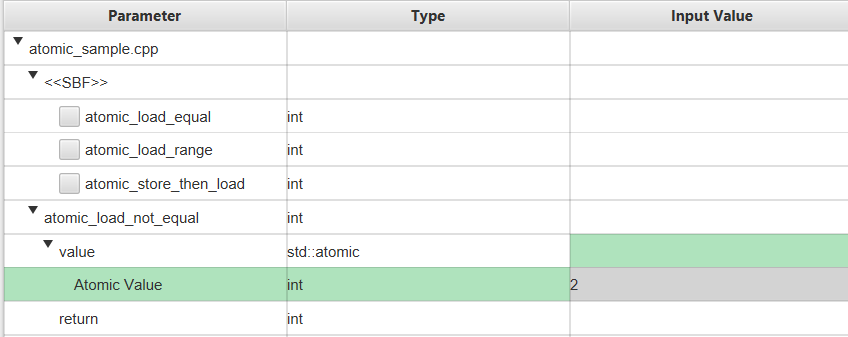
\includegraphics[width=0.9\textwidth]{images/atomic_after.png}
    \caption{AKAUTAUTO đã có thể nhận biết được trên Data Tree}
\end{figure}

Bên cạnh đó, cơ chế sinh test driver cũng được điều chỉnh nhằm xử lý đúng ngữ nghĩa của thư viện \texttt{std::atomic}. Thay vì sử dụng phép gán trực tiếp như đối với các kiểu dữ liệu thông thường, hệ thống sinh các câu lệnh \texttt{store()} để khởi tạo giá trị và sử dụng cặp thao tác \texttt{load()}--\texttt{store()} khi cần sao chép dữ liệu giữa các đối tượng nguyên tử. Nhờ đó, các đoạn mã kiểm thử được sinh ra có thể biên dịch và thực thi thành công đối với các hàm có tham số hoặc biến sử dụng \texttt{std::atomic}.

Kết quả thực nghiệm cho thấy phiên bản mở rộng của AKAUTAUTO có khả năng xử lý thành công các chương trình sử dụng \texttt{std::atomic}, bao gồm các trường hợp truyền tham chiếu, con trỏ, bí danh kiểu dữ liệu và các thao tác nguyên tử phổ biến như \texttt{load()}, \texttt{store()}, \texttt{exchange()} và \texttt{compare\_exchange()}.

\section{Dữ liệu và quy trình thực nghiệm}

\subsection{Dữ liệu thực nghiệm}

Để đánh giá tính đúng đắn của cơ chế hỗ trợ \texttt{std::atomic}, nghiên cứu xây dựng một bộ chương trình C++ thực nghiệm gồm 25 hàm sử dụng đối tượng nguyên tử dưới nhiều hình thức khác nhau. Các hàm được thiết kế nhằm kiểm tra khả năng nhận diện kiểu dữ liệu, xây dựng cây dữ liệu kiểm thử, sinh test driver và thực thi kiểm thử của hệ thống.

Bộ thực nghiệm được chia thành các nhóm chính bao gồm:

\begin{itemize}
\item Nhóm sử dụng các thao tác cơ bản \texttt{load()} và \texttt{store()}.
\item Nhóm sử dụng tham chiếu và con trỏ tới đối tượng \texttt{std::atomic}.
\item Nhóm sử dụng các bí danh kiểu dữ liệu như \texttt{std::atomic\_int}, \texttt{typedef} và \texttt{using}.
\item Nhóm sử dụng \texttt{std::atomic} làm thành viên của \texttt{struct} hoặc \texttt{class}.
\item Nhóm sử dụng các thao tác nguyên tử mở rộng như \texttt{exchange()}, nhóm \nolinkurl{fetch_*} và \nolinkurl{compare_exchange()}.
\item Nhóm kiểm thử cơ chế sinh stub và xử lý tham số kiểu \texttt{std::atomic}.
\end{itemize}

Các chương trình thực nghiệm được sử dụng để kiểm tra khả năng nhận diện đối tượng nguyên tử trong AST, xây dựng \texttt{AtomicDataNode}, sinh mã kiểm thử và thu thập kết quả độ phủ mã nguồn sau khi thực thi.


\subsection{Quy trình thực nghiệm}

\begin{table}[H]
\centering
\caption{Quy trình thực nghiệm nhận diện và biểu diễn \texttt{std::atomic}}
\label{tab:atomic-datanode-testing}
\renewcommand{\arraystretch}{1.3}
\begin{tabular}{@{}L{4cm}L{9cm}@{}}
\toprule
\multicolumn{2}{c}{\textbf{Testing Summary}} \\
\midrule
\textbf{Module} & Nhận diện \texttt{std::atomic} và xây dựng \texttt{AtomicDataNode} \\
\midrule
\textbf{Input} & Source code chứa biến hoặc tham số kiểu \texttt{std::atomic} \\
\midrule
\textbf{Expected output} &
\begin{minipage}[t]{\linewidth}
\raggedright
\vspace{-0.65\baselineskip}
\begin{itemize}
    \setlength{\itemsep}{2pt}
    \setlength{\parskip}{0pt}
    \setlength{\topsep}{0pt}
    \item Nhận diện đúng đối tượng \texttt{std::atomic}
    \item Tạo nút \texttt{AtomicDataNode} trong Data Tree
    \item Cho phép cấu hình giá trị kiểm thử cho kiểu dữ liệu cơ sở
\end{itemize}
\vspace{0.1\baselineskip}
\end{minipage} \\
\midrule
\textbf{Quy trình thực hiện} &
\begin{minipage}[t]{\linewidth}
\raggedright
\vspace{-0.65\baselineskip}
\begin{enumerate}
    \setlength{\itemsep}{2pt}
    \setlength{\parskip}{0pt}
    \setlength{\topsep}{0pt}
    \item Build môi trường kiểm thử
    \item Phân tích mã nguồn và xây dựng Data Tree
    \item Kiểm tra kiểu node được sinh ra cho đối tượng \texttt{atomic}
\end{enumerate}
\vspace{0.1\baselineskip}
\end{minipage} \\
\bottomrule
\end{tabular}
\end{table}

\textbf{Kịch bản 1: Nhận diện và biểu diễn đối tượng \texttt{std::atomic}.} Trong kịch bản này, dữ liệu đầu vào là các tệp mã nguồn có chứa biến hoặc tham số kiểu \texttt{std::atomic}. Hệ thống được kỳ vọng nhận diện đúng kiểu dữ liệu nguyên tử trong quá trình phân tích AST, xác định kiểu dữ liệu cơ sở và tạo nút \texttt{AtomicDataNode} tương ứng trong Data Tree. Người dùng sau đó có thể cấu hình giá trị kiểm thử cho đối tượng nguyên tử trên giao diện của công cụ.

\begin{table}[H]
\centering
\caption{Quy trình thực nghiệm sinh mã kiểm thử cho \texttt{std::atomic}}
\label{tab:atomic-driver-testing}
\renewcommand{\arraystretch}{1.3}
\begin{tabular}{@{}L{4cm}L{9cm}@{}}
\toprule
\multicolumn{2}{c}{\textbf{Testing Summary}} \\
\midrule
\textbf{Module} & Sinh test driver cho đối tượng \texttt{std::atomic} \\
\midrule
\textbf{Input} & Data Tree chứa \texttt{AtomicDataNode} và giá trị kiểm thử \\
\midrule
\textbf{Expected output} &
\begin{minipage}[t]{\linewidth}
\raggedright
\vspace{-0.6\baselineskip}
\begin{itemize}
    \setlength{\itemsep}{2pt}
    \setlength{\parskip}{0pt}
    \setlength{\topsep}{0pt}
    \item Sinh mã khởi tạo bằng \texttt{store()}
    \item Sao chép dữ liệu nguyên tử bằng \texttt{load()} và \texttt{store()}
    \item Biên dịch, thực thi và tạo báo cáo thành công
\end{itemize}
\vspace{0.4\baselineskip}
\end{minipage} \\
\midrule
\textbf{Quy trình thực hiện} &
\begin{minipage}[t]{\linewidth}
\raggedright
\vspace{-0.6\baselineskip}
\begin{enumerate}
    \setlength{\itemsep}{2pt}
    \setlength{\parskip}{0pt}
    \setlength{\topsep}{0pt}
    \item Tạo ca kiểm thử cho hàm sử dụng \texttt{std::atomic}
    \item Sinh test driver tự động
    \item Biên dịch và thực thi ca kiểm thử
    \item Thu thập báo cáo độ phủ mã nguồn
\end{enumerate}
\vspace{0.4\baselineskip}
\end{minipage} \\
\bottomrule
\end{tabular}
\end{table}

\textbf{Kịch bản 2: Sinh mã kiểm thử cho đối tượng \texttt{std::atomic}.} Kịch bản thứ hai tập trung đánh giá mã kiểm thử được sinh ra sau khi người dùng cấu hình dữ liệu cho đối tượng nguyên tử. Hệ thống cần sinh đúng khai báo biến \texttt{std::atomic}, sử dụng \texttt{store()} để khởi tạo giá trị và sử dụng \texttt{load()}--\texttt{store()} trong các ngữ cảnh sao chép dữ liệu. Kết quả kỳ vọng là mã sinh ra có thể biên dịch, thực thi thành công và tạo báo cáo độ phủ mã nguồn.

\section{Kết quả thực nghiệm}

Bảng~\ref{tab:atomic-testing-summary} trình bày các nhóm chức năng được sử dụng trong bộ thực nghiệm.


\begin{table}[H]
\centering
\caption{Các nhóm hàm thực nghiệm sử dụng \texttt{std::atomic}}
\label{tab:atomic-testing-summary}
\renewcommand{\arraystretch}{1.3}
\begin{tabular}{@{}cL{6cm}c@{}}
\toprule
\textbf{STT} & \textbf{Nhóm chức năng} & \textbf{Số hàm} \\
\midrule
1 & \texttt{load()} và \texttt{store()} & 4 \\
\midrule
2 & Atomic pointer và reference & 3 \\
\midrule
3 & Alias kiểu dữ liệu (\nolinkurl{atomic_int}, \texttt{typedef}, \texttt{using}) & 4 \\
\midrule
4 & Atomic trong \texttt{struct}/\texttt{class} & 4 \\
\midrule
5 & Các thao tác nguyên tử mở rộng (\texttt{exchange}, \nolinkurl{fetch_*}, \nolinkurl{compare_exchange}) & 7 \\
\midrule
6 & Stub liên quan đến \texttt{atomic} & 3 \\
\midrule
\multicolumn{2}{c}{\textbf{Tổng số hàm}} & \textbf{25} \\
\bottomrule
\end{tabular}
\end{table}

Kết quả thực nghiệm cho thấy hệ thống nhận diện thành công các đối tượng \texttt{std::atomic} trong tất cả các chương trình thử nghiệm, đồng thời xây dựng được nút \texttt{AtomicDataNode} tương ứng trong cây dữ liệu kiểm thử. Người dùng có thể cấu hình giá trị cho đối tượng nguyên tử thông qua giao diện Data Tree tương tự các kiểu dữ liệu đã được hỗ trợ trước đó.

\begin{figure}[H]
\centering
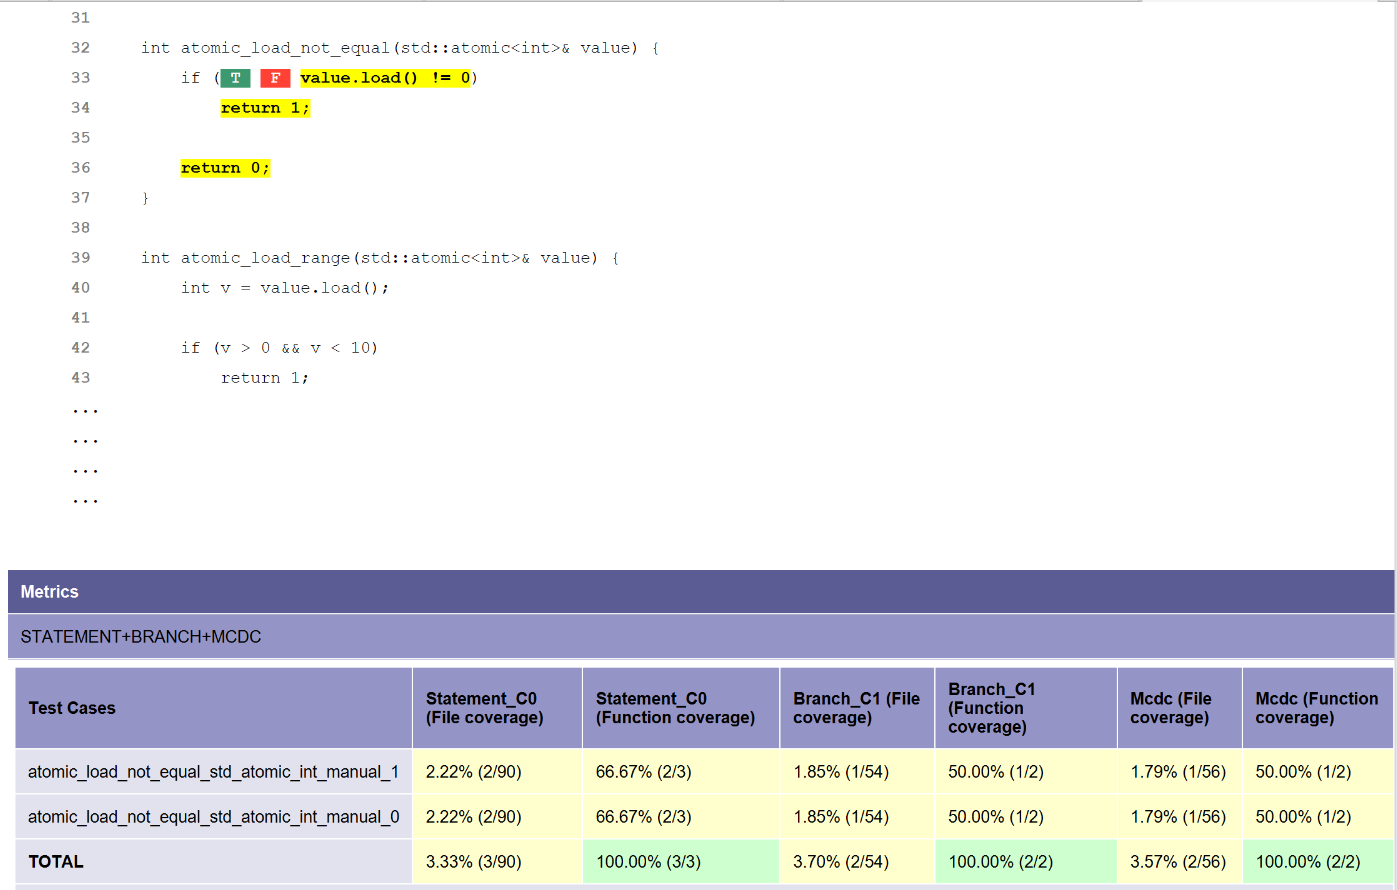
\includegraphics[width=0.9\textwidth]{images/atomic_execution.png}
\caption[Kết quả thực thi và độ phủ mã nguồn]{Kết quả thực thi và độ phủ mã nguồn của một hàm sử dụng \texttt{std::atomic}}
\label{fig:atomic_coverage}
\end{figure}


Đối với quá trình sinh test driver, hệ thống tạo thành công các câu lệnh khởi tạo sử dụng \texttt{store()} và xử lý việc sao chép dữ liệu nguyên tử thông qua cặp thao tác \texttt{load()}--\texttt{store()}. Các test driver được sinh ra đều có thể biên dịch và thực thi thành công trên các chương trình thực nghiệm.

Kết quả độ phủ mã nguồn cho thấy các nhánh điều kiện phụ thuộc vào giá trị của đối tượng \texttt{std::atomic} có thể được kích hoạt thông qua dữ liệu kiểm thử do người dùng cấu hình. Điều này chứng minh rằng cơ chế \texttt{AtomicDataNode} và các cải tiến trong bộ sinh test driver đã giúp AKAUTAUTO mở rộng phạm vi hỗ trợ đối với các chương trình sử dụng đối tượng nguyên tử.
